\documentclass[12pt, letterpaper, twoside]{article}
\usepackage{graphicx}
\graphicspath{ {./images/} }
\usepackage[utf8]{inputenc}
\usepackage{listings}
\usepackage{color}
\usepackage{tikz,pgfplots}

\definecolor{dkgreen}{rgb}{0,0.6,0}
\definecolor{gray}{rgb}{0.5,0.5,0.5}
\definecolor{mauve}{rgb}{0.58,0,0.82}

\lstset{frame=tb,
  language=C,
  aboveskip=2mm,
  belowskip=2mm,
  showstringspaces=false,
  columns=flexible,
  basicstyle={\small\ttfamily},
  numbers=none,
  numberstyle=\tiny\color{gray},
  keywordstyle=\color{blue},
  commentstyle=\color{dkgreen},
  stringstyle=\color{mauve},
  breaklines=true,
  breakatwhitespace=true,
  tabsize=2
}
\title{%
Design and Analysis of Algorithms\\
\large Graphs 3: Depth-First Search
}
\author{Daniel Shannon}
\date{April 21st, 2022}

\begin{document}

\begin{titlepage}
\maketitle
\end{titlepage}
\section*{3.3.3}
\begin{quote}
    For all nodes u,v, either [pre[u], post[u]] is completely within [pre[v], post[v]], or the other way around, or there is no overlap. Why?
    pre[u] to post[u] is the time u is on the stack.
\end{quote}
This is because each [pre[u],post[u]] is completely within [pre[v],post[v]] because only unexplored nodes are added to the stack.
So, when a node is added to the stack (u), all of the nodes for (v) will be discovered before the stack is emptied and returns to u. This is because v cannot be added to the exploration of u.
The name depth-first sort of implies this, too. If we start at a node (u), we search as deep as we can before returning to u, so any v searches will take less time than u.
\section*{3.3.5}
\begin{quote}
  What is the running time of DFS?
\end{quote}
The running time of DFS is O(N)
\begin{lstlisting}
procedure explore(G,v)
Input:  G(V,E) is a graph; v is in V
Output: visited(u) is set to true for all nodes u reachable from v
  previsit(v)                       //c1
  visisted(v)=true                  //c2
  for each edge (v,u) in E:         //N(E)
    if not visited(u): explore(u)   //c3
  postvisit(v)
\end{lstlisting}
It appears that the running time is $O(N)$, or or $O(E)$, since we call explore on depending on the size of the Edges.
Each edge is explored 1 time!
\section*{3.3.7}
\begin{quote}
Suppose that we start the explore procedure at node u. Use induction to prove that it will find all nodes reachable from u. Induction refresher: Prove the base case, then state the induction hypothesis, then do the inductive step.
\end{quote}

\textbf{Claim:} All nodes $v$ that are $k\ge0$ steps from $u$ can be found with the explore procedure.

\textbf{Base Case:} For $k=0$, $explore(k=0)$ discovers $u=v$ immediately, and $k\ge0$ nodes will be discovered, too.

\textbf{Proof by Induction:} For $k+1$, $u[k+1]$ will be discovered as $v[k+1]$. Through induction all nodes for $k\ge{0}$ will be discovered through explore.
\section*{3.3.9}
\begin{enumerate}
  \item How many parents can a node have in the DFS tree?
  
  A node can have one parent because it can only be marked as visited coming from one other node.
  
  \item How many children can a node have in the DFS tree?
  
  A node can have as many children as there are nodes coming from that node.
  
  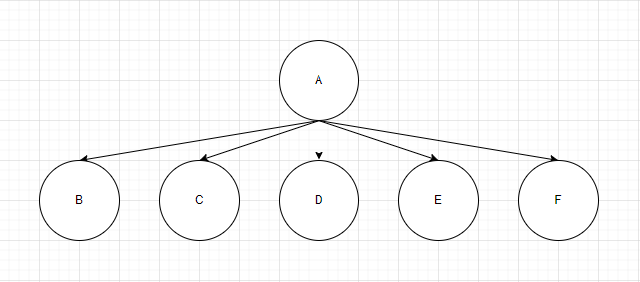
\includegraphics[]{dfsManyChildren.png}

  \item How many ancestors can a node have in the DFS tree?
  
  If there are $k$ nodes in a graph, the DFS could have up to $k-2$ ancestors - the total number of nodes minus the parent and the bottom most node.

  \item How many descendants can a node have in the DFS tree?
  
  A node can have $k-1$ nodes when there are $k$ nodes in the graph. This is assuming the graph is essentially a linked list.

\end{enumerate}
\end{document}